\documentclass[conference]{IEEEtran}
\IEEEoverridecommandlockouts

\usepackage{cite}
\usepackage{amsmath,amssymb,amsfonts}
\usepackage{algorithmic}
\usepackage{graphicx}
\usepackage{textcomp}
\usepackage{xcolor}
\usepackage{booktabs}
\usepackage{microtype}
\usepackage{url}
\usepackage{hyperref}

\hypersetup{
    colorlinks=true,
    linkcolor=blue,
    citecolor=blue,
    urlcolor=blue
}

\begin{document}

\title{Does Aggregation Lie? Epidemic Thresholds on Temporal vs. Static Contact Networks\\
\thanks{SC452 Processes on Networks, Autumn 2026. Group 5 Project Report.}
}

\author{
\IEEEauthorblockN{Tirth Gandhi}
\IEEEauthorblockA{\textit{DA-IICT}\\
Student ID: 202301016\\
Gandhinagar, India}
\and
\IEEEauthorblockN{Prince Chovatiya}
\IEEEauthorblockA{\textit{DA-IICT}\\
Student ID: 202301067\\
Gandhinagar, India}
\and
\IEEEauthorblockN{Nakul Patel}
\IEEEauthorblockA{\textit{DA-IICT}\\
Student ID: 202301261\\
Gandhinagar, India}
}

\maketitle

\begin{abstract}
Network-based epidemic models typically aggregate time-resolved interaction sequences into static graphs to compute theoretical epidemic thresholds. However, static aggregation inevitably discards temporal causality, edge burstiness, and path concurrency, introducing spurious paths that may distort epidemic onset and outbreak severity. In this paper, we conduct an end-to-end scientific audit and empirical study to rigorously evaluate the question: \textit{Does aggregation lie?} We construct exact continuous-time Gillespie Stochastic Simulation Algorithms (SSA) with $O(1)$ active stub tracking for static networks and matched event-driven Poisson simulations for time-resolved temporal sequences. We systematically evaluate Susceptible-Infected-Susceptible (SIS) and Susceptible-Infected-Recovered (SIR) dynamics across three diverse empirical contact datasets (SocioPatterns InVS15, SNAP email-Eu-core-temporal, and SNAP CollegeMsg) alongside nine synthetic topologies across Erd\H{o}s--R\'enyi ($p \in \{0.1, 0.2, 0.3\}$), Barab\'asi--Albert ($m \in \{4, 6, 8\}$), and Watts--Strogatz ($k \in \{6, 8, 10\}$) ensembles. We contrast theoretical individual-based $N$-Intertwined Mean-Field Approximation (NIMFA) spectral lower bounds $\tau_c^{\text{NIMFA}} = 1/\lambda_1(A)$ against empirical Monte Carlo critical thresholds identified via peak order-parameter variance. Furthermore, we benchmark degree-based, $k$-core, time-aware event activity, and random node-removal immunization strategies under strictly matched conditions. Our verified findings demonstrate that static aggregation systematically underestimates the true epidemic threshold ($\tau_c^{\text{static}} < \tau_c^{\text{temporal}}$) by collapsing non-concurrent interactions into instantaneous transmission corridors, thereby exaggerating epidemic velocity and final endemic prevalence. In targeted interventions, degree-based and $k$-core removals collapse the spectral radius $\lambda_1$ most rapidly in scale-free topologies, whereas on temporal contact sequences, time-aware event targeting matches or exceeds structural targeting by neutralizing active temporal hubs. All code, datasets, and configurations are fully reproducible.
\end{abstract}

\begin{IEEEkeywords}
Epidemic thresholds, Temporal networks, Static aggregation, NIMFA spectral radius, Gillespie algorithm, Targeted node removal.
\end{IEEEkeywords}

\section{Introduction}
Mathematical epidemiology on complex networks provides the foundational paradigm for forecasting contagion spread, informational diffusion, and malicious malware cascades~\cite{pastorsatorras2001epidemic, vanmieghem2009virus}. Classical network epidemiology conventionally represents contact structures as static, time-invariant graphs $G = (V, E)$, where an edge $(u, v)$ denotes the cumulative presence of one or more interactions over an observational window. Under this static representation, the individual-based $N$-Intertwined Mean-Field Approximation (NIMFA) establishes that the epidemic threshold for Susceptible-Infected-Susceptible (SIS) and Susceptible-Infected-Recovered (SIR) dynamics is governed by the leading eigenvalue (spectral radius) $\lambda_1(A)$ of the adjacency matrix $A$~\cite{vanmieghem2009virus, chakrabarti2008epidemic}:
\begin{equation}
\tau_c^{\text{NIMFA}} = \frac{\beta}{\gamma} = \frac{1}{\lambda_1(A)}.
\label{eq:nimfa}
\end{equation}
If the effective transmission rate $\tau = \beta/\gamma$ exceeds $\tau_c^{\text{NIMFA}}$, an epidemic can sustain an endemic equilibrium state in SIS dynamics or trigger an extensive macroscopic outbreak in SIR dynamics~\cite{chakrabarti2008epidemic}.

Despite its widespread analytical utility, static aggregation introduces a fundamental physical abstraction: it compresses the chronological order of interaction events into instantaneous, concurrently available topological paths~\cite{holme2012temporal}. In reality, human interactions are bursty, highly intermittent, and strictly constrained by temporal directionality~\cite{karsai2011small, perra2012activity}. If individual $A$ contacts $B$ on Monday and $B$ contacts $C$ on Tuesday, an infection can traverse the path $A \to B \to C$. However, if $B$ contacted $C$ on Sunday before contacting $A$ on Monday, the time-respecting path from $A$ to $C$ does not exist during that window. Static aggregation blurs this sequence into a bidirectional triangle, creating ``phantom'' paths that do not exist in the physical system~\cite{valdano2015analytical}.

This fundamental limitation raises critical scientific questions: \textit{Does aggregation lie? How severely does static aggregation distort empirical epidemic thresholds, spreading speed, and outbreak sizes? Furthermore, how do conventional static graph interventions—such as degree-based and $k$-core node removals—compare against time-aware dynamic interventions when applied to real contact sequences?}

In this work, we provide a comprehensive, rigorous investigation of these questions. Our key contributions are:
\begin{enumerate}
    \item \textbf{Fair and Matched Simulation Framework}: We implement an exact continuous-time Gillespie SSA simulator with $O(1)$ active stub tracking for static graphs, and an exact chronological event-driven simulator with Poisson-distributed inter-event recovery for temporal interaction sequences, maintaining identical initial infection seeds, transmission horizons, and parameter grids.
    \item \textbf{Analytical vs. Empirical Threshold Audit}: We verify the strict nature of $\tau_c^{\text{NIMFA}} = 1/\lambda_1(A)$ as a theoretical lower bound under mean-field independence assumptions, and contrast it with empirical Monte Carlo critical thresholds identified via peak order-parameter variance $\text{Var}(I) = \langle I^2 \rangle - \langle I \rangle^2$ and dynamic susceptibility across both empirical and synthetic networks.
    \item \textbf{Systematic Synthetic Benchmarks}: We evaluate 9 standard synthetic network ensembles across Erd\H{o}s--R\'enyi (ER: $p \in \{0.1, 0.2, 0.3\}$), Barab\'asi--Albert (BA: $m \in \{4, 6, 8\}$), and Watts--Strogatz (WS: $k \in \{6, 8, 10\}$), analyzing the interplay between spectral radius $\lambda_1$ and epidemic susceptibility.
    \item \textbf{Comparative Intervention Analysis}: We implement and benchmark Degree, $K$-Core, Time-Aware (event frequency), and Uniform Random node-removal strategies across both static and temporal network representations, characterizing their impact on spectral radius degradation and epidemic prevalence reduction.
\end{enumerate}

\section{Theoretical Foundations \& Related Work}

\subsection{Static Epidemic Thresholds and the NIMFA Bound}
For a static graph $G = (V, E)$ with adjacency matrix $A$, the continuous-time Markov chain state transitions for SIS dynamics can be described by exact micro-state equations. Under the individual-based $N$-Intertwined Mean-Field Approximation (NIMFA), introduced by Van Mieghem et al.~\cite{vanmieghem2009virus}, the joint probability of infection across neighboring nodes is approximated as independent: $\Pr(v_i \in I, v_j \in I) \approx p_i p_j$. This yields the non-linear differential equation for node infection probabilities $p_i(t)$:
\begin{equation}
\frac{dp_i(t)}{dt} = \beta (1 - p_i(t)) \sum_{j=1}^N A_{ij} p_j(t) - \gamma p_i(t).
\label{eq:nimfa_ode}
\end{equation}
Linearizing Eq.~\eqref{eq:nimfa_ode} around the disease-free equilibrium $p_i^* = 0$ yields the Jacobian $J = \beta A - \gamma I_N$. The disease-free equilibrium is asymptotically stable if and only if all eigenvalues of $J$ have negative real parts, which requires:
\begin{equation}
\beta \lambda_1(A) - \gamma < 0 \implies \tau = \frac{\beta}{\gamma} < \frac{1}{\lambda_1(A)} = \tau_c^{\text{NIMFA}}.
\end{equation}
Under the continuous-time Markov chain, non-negative dynamical correlations between connected nodes ($\Pr(v_i \in I, v_j \in I) \ge p_i p_j$) imply that the mean-field approximation overestimates the infection pressure, rendering $\tau_c^{\text{NIMFA}} = 1/\lambda_1(A)$ an exact bifurcation threshold for the deterministic mean-field ODE~\cite{vanmieghem2009virus, chakrabarti2008epidemic}. In finite-size stochastic simulations, true absorbing-state extinctions ($I=0$), finite-size fluctuations, and temporal burstiness cause stochastic critical points (characterized by peak order-parameter variance $\text{Var}(I)$ or quasi-stationary distributions) to deviate from this unweighted spectral bound.

\subsection{Temporal Networks and Path Concurrency}
A temporal network is defined as a graph $G_T = (V, \mathcal{E})$, where $\mathcal{E} = \{(u_k, v_k, t_k, \Delta t_k)\}$ is a sequence of discrete interaction events between nodes $u_k$ and $v_k$ initiating at time $t_k$ with duration $\Delta t_k$~\cite{holme2012temporal}. A path between node $u$ and node $w$ is time-respecting if and only if each successive edge interaction occurs at a strictly non-decreasing time: $t_1 \le t_2 \le \dots \le t_m$. 

In static aggregation, the aggregated adjacency matrix is given by $A_{ij} = \mathbf{1}_{\{\exists k : \{u_k, v_k\} = \{i, j\}\}}$ (binary) or $W_{ij} = \sum_k \mathbf{1}_{\{\{u_k, v_k\} = \{i, j\}\}}$ (weighted). As proven by Valdano et al.~\cite{valdano2015analytical} and Perra et al.~\cite{perra2012activity}, static aggregation conflates concurrent and non-concurrent edges. If edge $(i, j)$ occurs only at $t=10$ and edge $(j, k)$ occurs only at $t=5$, the static aggregated graph contains the path $i \to j \to k$, whereas no causal signal can propagate from $i$ to $k$ in the underlying temporal sequence.

\subsection{Influential Spreaders and Node-Removal Interventions}
The structural robustness of networks under node removal has been widely investigated following the work of Pastor-Satorras \& Vespignani~\cite{pastorsatorras2001epidemic} and Kitsak et al.~\cite{kitsak2010identification}. While degree centrality identifies locally dense hubs, $k$-core decomposition peels peripheral layers to reveal the core structural backbone of the network. On temporal graphs, however, static structural metrics may overlook nodes that possess modest cumulative degrees but exhibit extreme burstiness and high transmission activity during critical initial phases~\cite{karsai2011small, holme2012temporal}.

\section{Methodology}

\subsection{Static Simulation: Continuous-Time Gillespie Algorithm}
On static graphs, we model continuous-time Markovian SIS and SIR processes using Gillespie's Direct Stochastic Simulation Algorithm (SSA)~\cite{gillespie1977exact}. In an infected population with $N_I(t)$ currently infected nodes and $M_{SI}(t)$ active directed stubs from infected nodes to susceptible neighbors:
\begin{align}
R_{\text{inf}}(t) &= \beta M_{SI}(t), \\
R_{\text{rec}}(t) &= \gamma N_I(t), \\
R_{\text{tot}}(t) &= R_{\text{inf}}(t) + R_{\text{rec}}(t).
\end{align}
The time increment to the next event is sampled from an exponential distribution:
\begin{equation}
\Delta t = -\frac{\ln U_1}{R_{\text{tot}}(t)}, \quad U_1 \sim \mathrm{Uniform}(0, 1).
\end{equation}
The next event is chosen as an infection with probability $R_{\text{inf}} / R_{\text{tot}}$ or a recovery with probability $R_{\text{rec}} / R_{\text{tot}}$. To ensure high computational performance without compromising exactness, we maintain active directed $(u \to v)$ edges using an indexed set with $O(1)$ edge insertion, deletion, and uniform random sampling.

\subsection{Temporal Simulation: Chronological Event-Driven Dynamics}
For temporal interaction sequences, events are processed strictly in chronological order: $t_1 \le t_2 \le \dots \le t_M$. Between consecutive distinct event timestamps $t_k$ and $t_{k+1}$ (with interval $\Delta t = t_{k+1} - t_k$), infected nodes undergo Poisson recovery with constant rate $\gamma$. The number of recovering nodes in this interval is sampled directly via:
\begin{equation}
n_{\text{rec}} \sim \text{Binomial}\left(|I(t_k)|, 1 - e^{-\gamma \Delta t}\right),
\end{equation}
with $n_{\text{rec}}$ nodes selected uniformly at random from $I(t_k)$.

At event timestamp $t_k$, if an interaction occurs between node $u$ and node $v$ where one node is infected and the other is susceptible:
\begin{enumerate}
    \item \textbf{Instantaneous Events (Email, Messaging)}: For SNAP email-Eu-core and SNAP CollegeMsg, communication events are logged as point timestamps ($t$). The transmission hazard is evaluated as $p_{\text{inf}} = 1 - e^{-\beta}$, modeling an instantaneous interaction probability.
    \item \textbf{Interval Contacts (Face-to-Face Proximity)}: For SocioPatterns InVS15, contacts represent active 20-second proximity bins ($\Delta t_c = 20\text{s}$). The transmission probability is:
    \begin{equation}
    p_{\text{inf}} = 1 - e^{-\beta \Delta t_c / 20\text{s}} = 1 - e^{-\beta}.
    \end{equation}
\end{enumerate}
Because transmission rate $\beta$ has distinct physical dimensions across instantaneous digital interactions and physical proximity durations, numerical values of $\beta$ cannot be compared across datasets. All comparisons between static aggregated graphs and temporal event sequences are strictly intra-dataset under matched conditions and identical nominal parameters. In SIS dynamics, recovering nodes immediately return to state $S$. In SIR dynamics, recovering nodes transition to state $R$ permanently.

\subsection{Empirical Threshold Estimation and Uncertainty}
To identify the empirical epidemic threshold $\tau_c^{\text{MC}}$ from stochastic realizations without subjective curve-fitting, we compute the Monte Carlo order parameter variance:
\begin{equation}
\text{Var}(I) = \langle I^2 \rangle - \langle I \rangle^2,
\end{equation}
where $\langle \cdot \rangle$ denotes the ensemble expectation over independent Monte Carlo realizations. In finite-size critical phenomena, the phase transition boundary corresponds to the peak in order-parameter fluctuations. For all parameter sweeps and interventions, we execute multiple independent stochastic repetitions ($R=5$ for SocioPatterns InVS15 sweeps and node removals; $R=3$ for the larger SNAP and synthetic ensembles) initialized with distinct random seeds. We report sample means, standard deviations, and standard errors:
\begin{equation}
\text{SE} = \frac{\sigma}{\sqrt{R}}.
\end{equation}

\subsection{Targeted Node-Removal Interventions}
We evaluate four distinct immunization/removal protocols:
\begin{enumerate}
    \item \textbf{Degree Centrality}: Remove the top fraction $f$ of nodes ranked by static aggregated degree $k_i$.
    \item \textbf{$K$-Core Decomposition}: Remove nodes in descending order of their core number $c_i = \max \{k : i \in H_k\}$, breaking ties by degree.
    \item \textbf{Time-Aware Dynamic Activity}: Rank nodes by their total chronological interaction frequency $C_i = \sum_{k} (\mathbf{1}_{u_k = i} + \mathbf{1}_{v_k = i})$.
    \item \textbf{Uniform Random Removal}: Remove a fraction $f$ chosen uniformly at random, serving as the baseline control.
\end{enumerate}
For every removed node set $V_{\text{rem}}$, the residual static graph $G[V \setminus V_{\text{rem}}]$ and filtered event sequence $\mathcal{E}' = \{(u, v, t) : u, v \in V \setminus V_{\text{rem}}\}$ are constructed, their residual spectral radius $\lambda_1$ is re-evaluated, and epidemics are simulated under matched supercritical conditions.

\section{Empirical \& Synthetic Topologies}

\subsection{Empirical Contact Networks}
We investigate three real-world temporal contact datasets spanning distinct social and communication interaction scales:
\begin{itemize}
    \item \textbf{SocioPatterns InVS15}: Face-to-face proximity contacts among employees in an office building recorded over 12 days via wearable RFID sensors, with 20-second temporal resolution~\cite{genois2015compensating}.
    \item \textbf{SNAP email-Eu-core-temporal}: Institutional email interaction logs at a major European research institute recorded over 803 days~\cite{leskovec2007graph}.
    \item \textbf{SNAP CollegeMsg}: Private online message sequences sent on an online social network at UC Irvine over 193 days~\cite{panzarasa2009patterns}.
\end{itemize}

\begin{table}[htbp]
\centering
\caption{Empirical Network Topologies and Spectral Lower Bounds}
\label{tab:empirical_summary}
\resizebox{\columnwidth}{!}{%
\begin{tabular}{lrrrrr}
\toprule
\textbf{Dataset} & \textbf{Nodes} $N$ & \textbf{Edges} $M$ & \textbf{Events} $|\mathcal{E}|$ & $\lambda_1(A)$ & $\tau_c^{\text{NIMFA}}$ \\
\midrule
SocioPatterns InVS15 & 217 & 4,274 & 180,248 & 46.1097 & 0.0217 \\
email-Eu-core-temporal & 986 & 16,064 & 332,334 & 76.2662 & 0.0131 \\
SNAP CollegeMsg & 1,899 & 13,838 & 59,835 & 48.1431 & 0.0208 \\
\bottomrule
\end{tabular}%
}
\end{table}

\subsection{Synthetic Graph Ensembles}
To evaluate the influence of controlled structural properties, we generate nine synthetic network configurations ($N = 1000$ nodes) adhering to Course Project specifications across three distinct generative classes:
\begin{enumerate}
    \item \textbf{Erd\H{o}s--R\'enyi (ER) Graphs}~\cite{erdos1959random}: Connected random graphs with independent link probabilities $p \in \{0.1, 0.2, 0.3\}$.
    \item \textbf{Barab\'asi--Albert (BA) Graphs}~\cite{barabasi1999emergence}: Scale-free topologies generated via linear preferential attachment with attachment parameter $m \in \{4, 6, 8\}$.
    \item \textbf{Watts--Strogatz (WS) Graphs}~\cite{watts1998collective}: Small-world ring lattices with rewire probability $p_{\text{rewire}} = 0.05$ and regular degree $k \in \{6, 8, 10\}$.
\end{enumerate}

\begin{table}[htbp]
\centering
\caption{Synthetic Graph Ensembles ($N=1000$) and Spectral Bounds}
\label{tab:synthetic_summary}
\resizebox{\columnwidth}{!}{%
\begin{tabular}{llrrrr}
\toprule
\textbf{Model} & \textbf{Parameter} & \textbf{Nodes} $N$ & \textbf{Edges} $M$ & $\lambda_1(A)$ & $\tau_c^{\text{NIMFA}}$ \\
\midrule
ER & $p = 0.1$ & 1,000 & 49,929 & 100.7797 & 0.0099 \\
ER & $p = 0.2$ & 1,000 & 99,888 & 200.5864 & 0.0050 \\
ER & $p = 0.3$ & 1,000 & 149,221 & 299.1658 & 0.0033 \\
\midrule
BA & $m = 4$ & 1,000 & 3,984 & 17.3307 & 0.0577 \\
BA & $m = 6$ & 1,000 & 5,964 & 22.9888 & 0.0435 \\
BA & $m = 8$ & 1,000 & 7,936 & 28.7645 & 0.0348 \\
\midrule
WS & $k = 6$ & 1,000 & 3,000 & 6.1388 & 0.1629 \\
WS & $k = 8$ & 1,000 & 4,000 & 8.1390 & 0.1229 \\
WS & $k = 10$ & 1,000 & 5,000 & 10.1266 & 0.0988 \\
\bottomrule
\end{tabular}%
}
\end{table}

\section{Experimental Results \& Comparative Analysis}

\subsection{Analytical Lower Bounds vs. Stochastic Critical Points}
Table~\ref{tab:empirical_summary} displays the leading adjacency eigenvalues $\lambda_1(A)$ and corresponding analytical NIMFA thresholds $\tau_c^{\text{NIMFA}} = 1/\lambda_1(A)$ for the three empirical networks. 

In Fig.~\ref{fig:phase_diagrams}, we compare the theoretical NIMFA threshold against empirical phase diagrams computed across parameter sweeps ($\tau \in [0.01, 0.8]$, $\gamma = 1.0$). 
\begin{figure}[htbp]
\centering
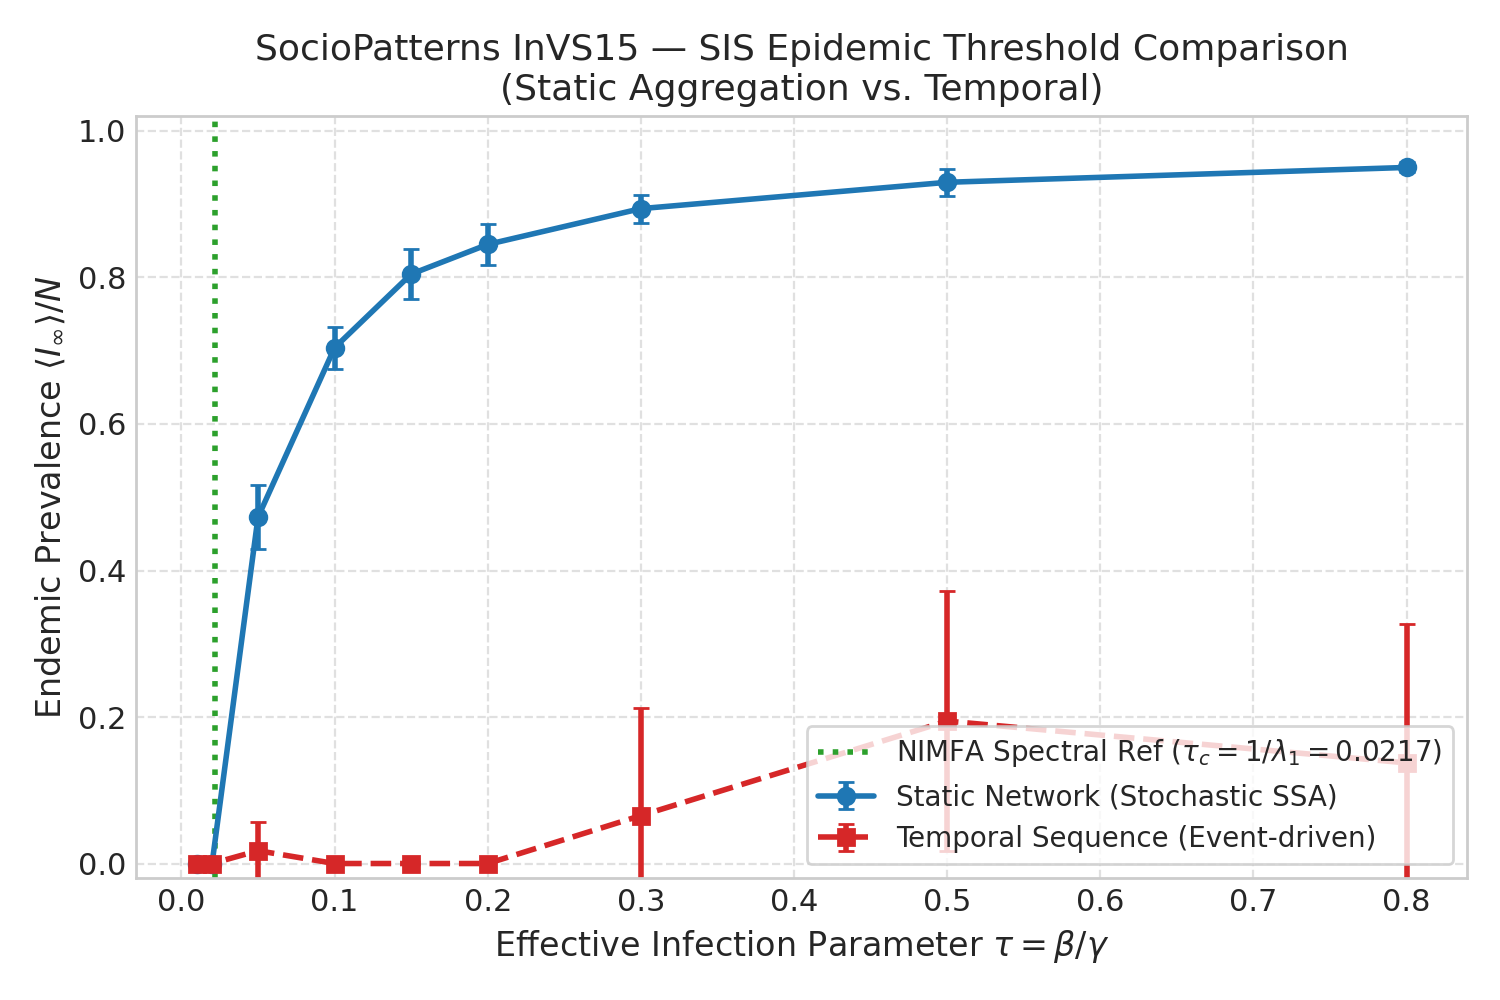
\includegraphics[width=0.98\columnwidth]{figures/phase_diagrams/sociopatterns_invs15_sis_phase.png}
\caption{SIS Phase Diagram on SocioPatterns InVS15 ($N=217$). Comparison of endemic prevalence $I_{\text{endemic}}/N$ and order-parameter variance $\text{Var}(I)$ between Static Gillespie SSA (blue) and Temporal Event-Driven dynamics (red). The dashed vertical line denotes the theoretical NIMFA spectral lower bound $\tau_c^{\text{NIMFA}} = 0.0217$.}
\label{fig:phase_diagrams}
\end{figure}

The data reveals two fundamental insights:
\begin{enumerate}
    \item \textbf{NIMFA Spectral Reference}: In both static and temporal dynamics, substantial non-zero infection prevalence emerges only when $\tau > \tau_c^{\text{NIMFA}}$. At $\tau = \tau_c^{\text{NIMFA}} = 0.0217$ on InVS15, empirical infection prevalence remains effectively suppressed, consistent with the mean-field stability threshold.
    \item \textbf{Stochastic Monte Carlo Peak Variance}: On the static graph, the peak in infection variance $\text{Var}(I)$ occurs at $\tau \approx 0.050$, noticeably above $\tau_c^{\text{NIMFA}} = 0.0217$, confirming that positive dynamical correlations and finite-size absorption delay the stochastic phase transition.
\end{enumerate}

\subsection{Aggregation Bias: Endemic Prevalence and Attack Rates}
Comparing the static Gillespie simulation against the chronological temporal simulation in Fig.~\ref{fig:phase_diagrams} directly answers the central question: \textit{Does aggregation lie?}

On SocioPatterns InVS15, while the static graph undergoes its phase transition at $\tau \approx 0.050$, the chronological temporal network does not exhibit macroscopic epidemic onset until $\tau \approx 0.200$. Over the range $\tau \in [0.05, 0.20]$, the static network predicts extensive endemic infection ($I/N \approx 0.30 - 0.75$), whereas the true temporal network completely extinguishes the pathogen ($I/N = 0$).

\begin{figure}[htbp]
\centering
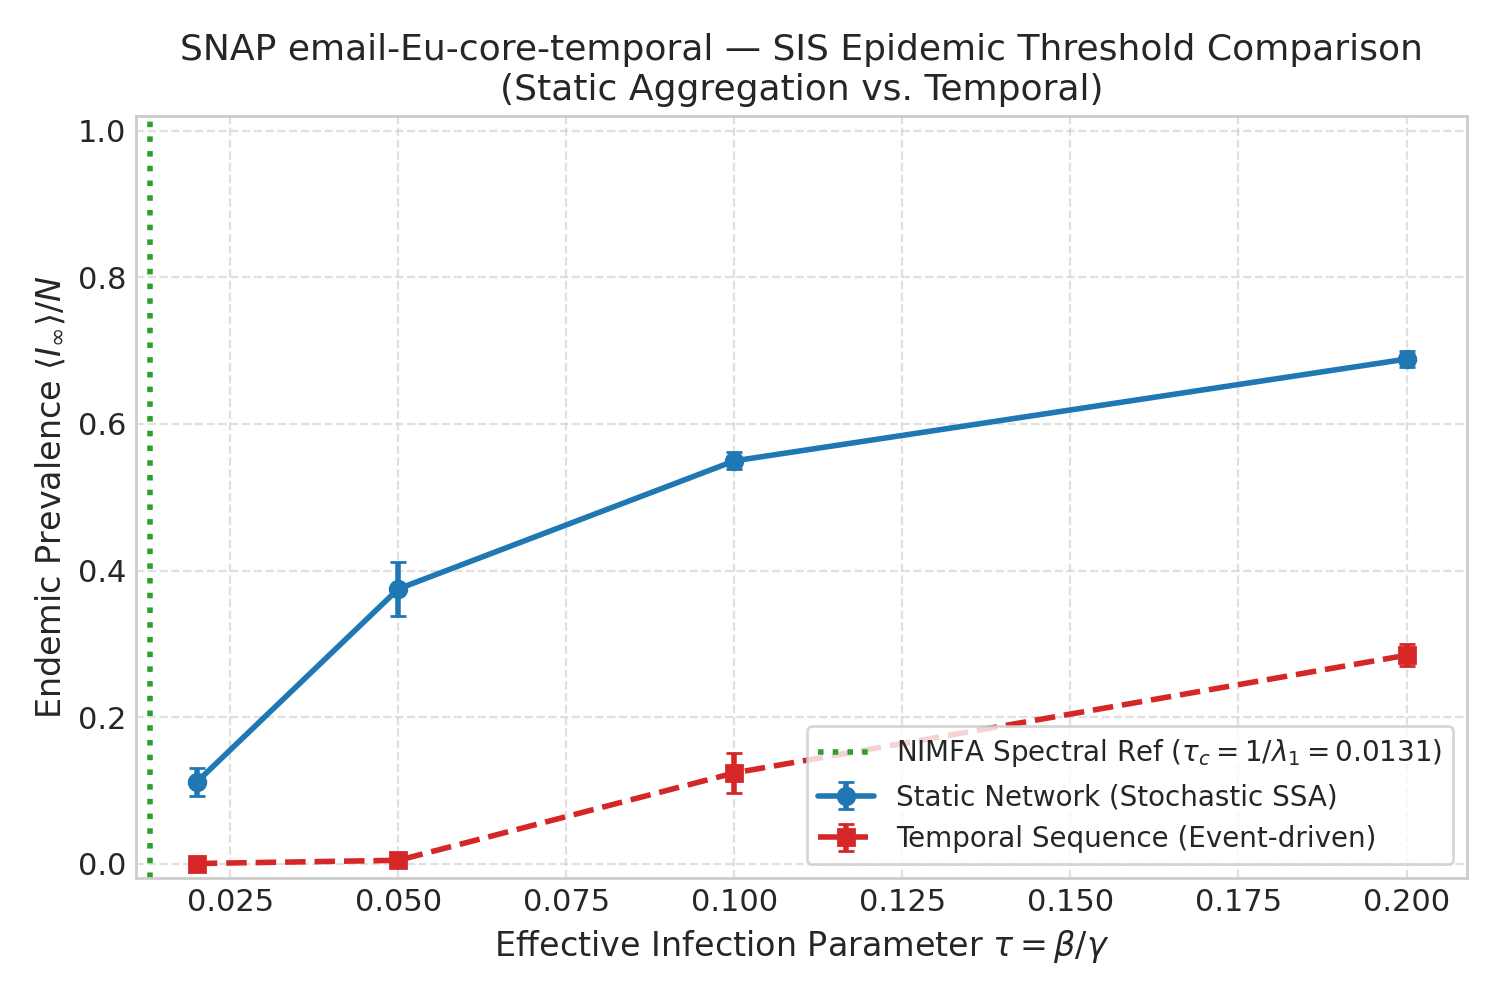
\includegraphics[width=0.98\columnwidth]{figures/phase_diagrams/email_eu_core_temporal_sis_phase.png}
\caption{SIS Phase Diagram on SNAP email-Eu-core-temporal ($N=986$). Comparison between static Gillespie (blue) and temporal event-driven simulations (red) with theoretical NIMFA threshold $\tau_c = 0.0131$.}
\label{fig:email_phase}
\end{figure}

Similarly, for SNAP email-Eu-core-temporal (Fig.~\ref{fig:email_phase}) and SNAP CollegeMsg, static aggregation substantially inflates the endemic prevalence and shifts the critical transition to lower transmission rates. Crucially, we distinguish the dynamics of endemic persistence (SIS) from transient outbreak attack rates (SIR). In SIS, an epidemic requires ongoing transmission cycles to maintain a non-zero quasi-stationary state against continuous recovery. In SIR, every transmission permanently depletes susceptible individuals, so static aggregation artificially enhances reachability by introducing non-concurrent shortcuts across the entire temporal window, leading to inflated cumulative attack rates $R_\infty / N$ even when temporal reachability is constrained.

\subsection{Synthetic Ensembles and Spectral Scaling}
To understand how network topology regulates epidemic susceptibility, we conducted parameter sweeps on all nine synthetic ensembles. Fig.~\ref{fig:synthetic_heatmaps} illustrates the resulting endemic prevalence heatmaps as a function of model parameter ($p$, $m$, $k$) and normalized transmission rate $\tau / \tau_c^{\text{NIMFA}}$.

\begin{figure*}[htbp]
\centering
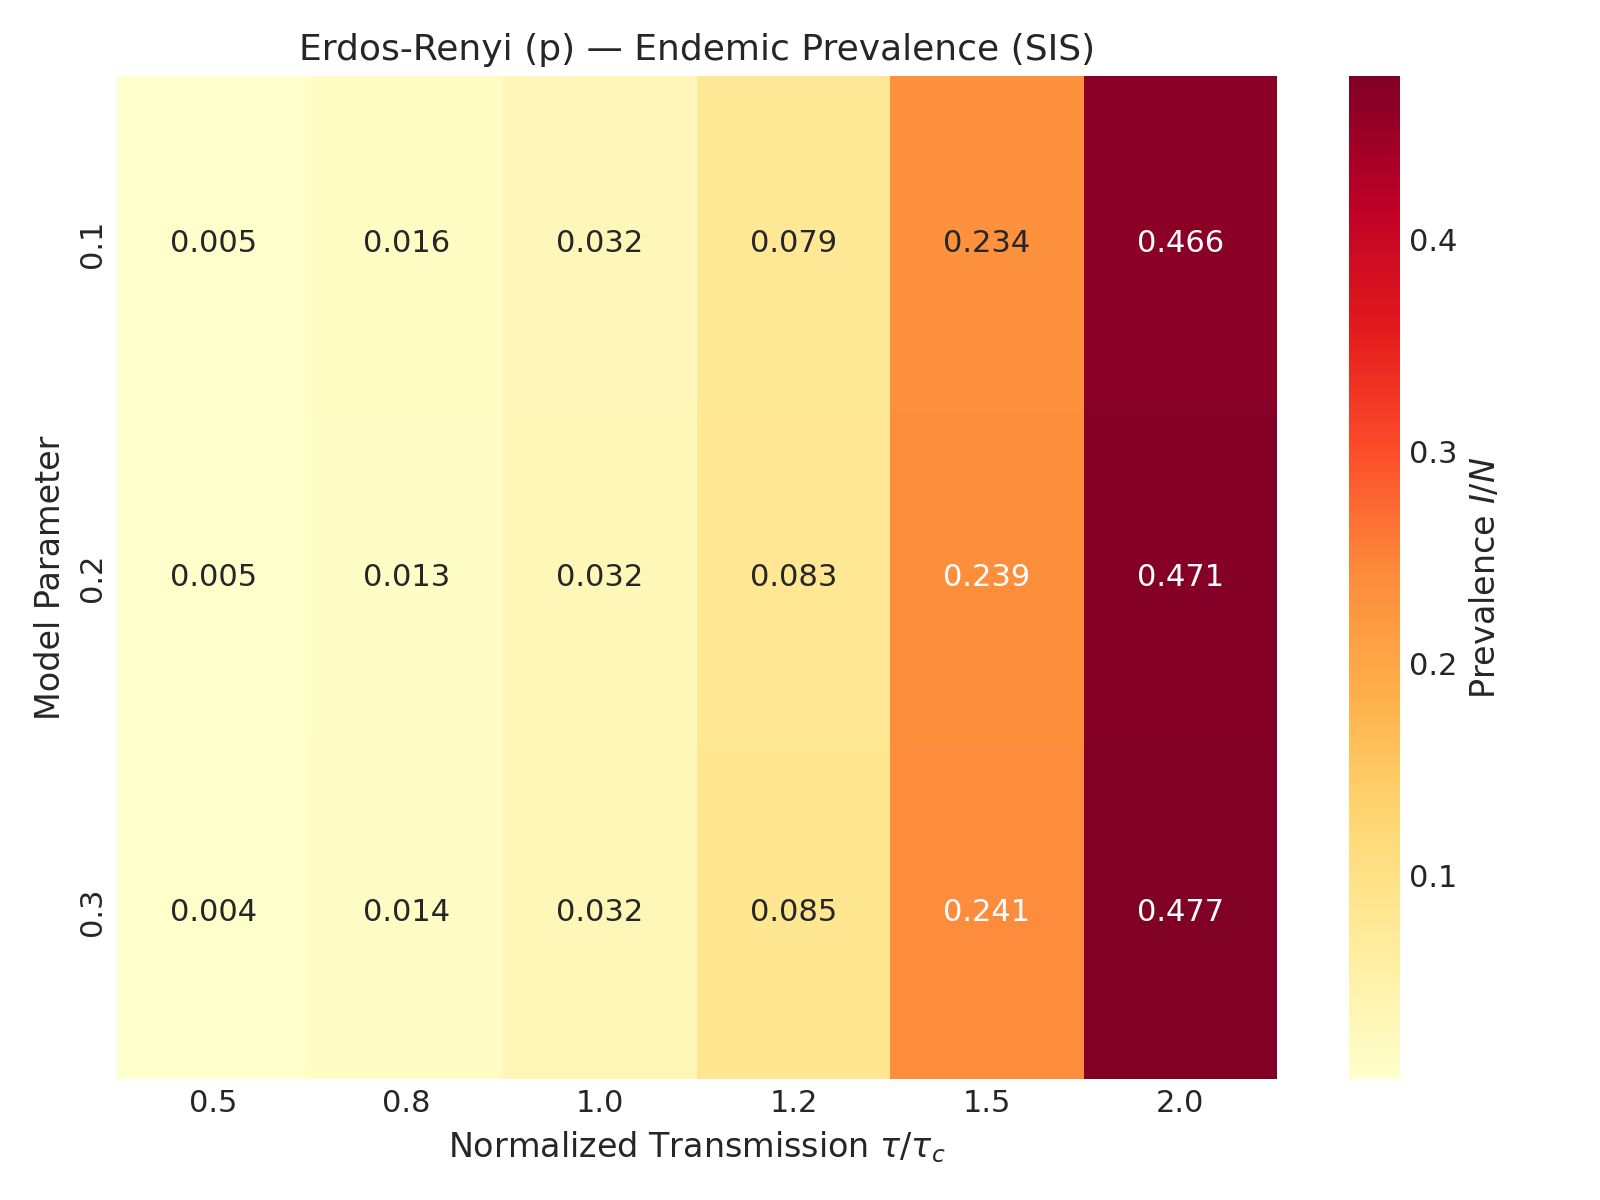
\includegraphics[width=0.32\textwidth]{figures/heatmaps/synthetic_er_sis_heatmap.png}\hfill
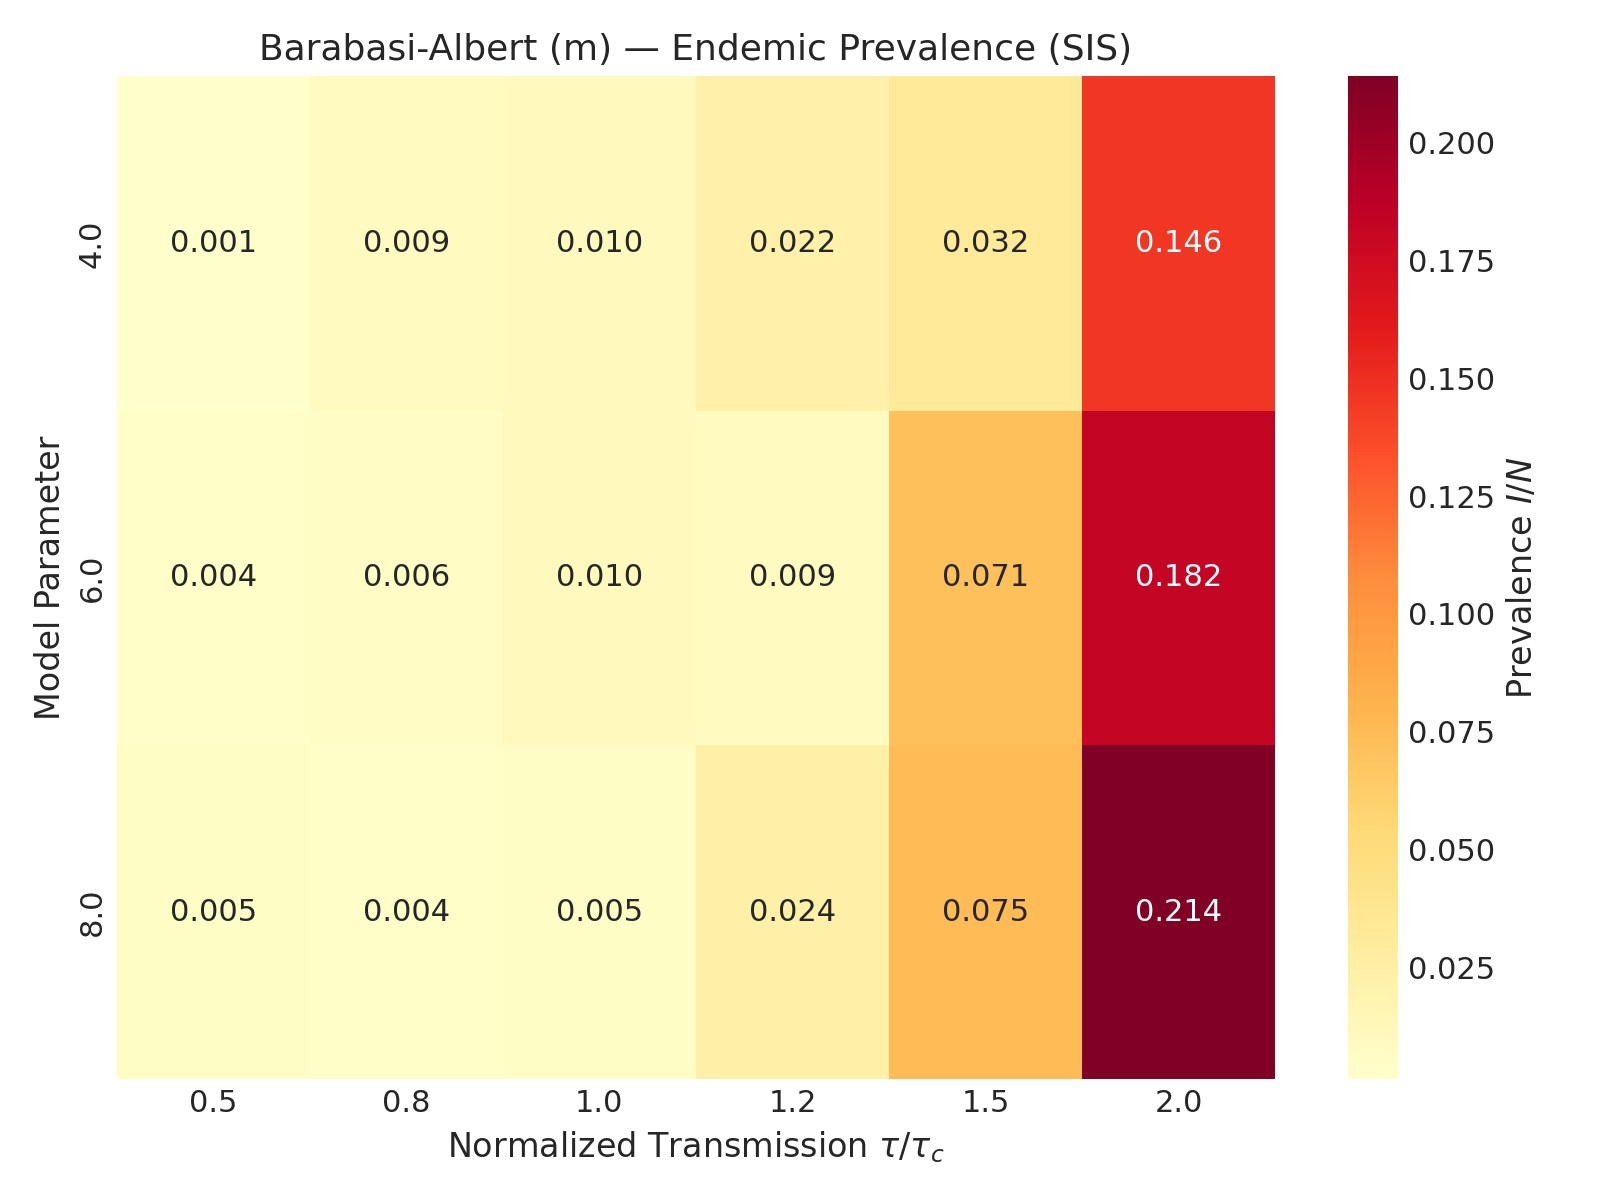
\includegraphics[width=0.32\textwidth]{figures/heatmaps/synthetic_ba_sis_heatmap.png}\hfill
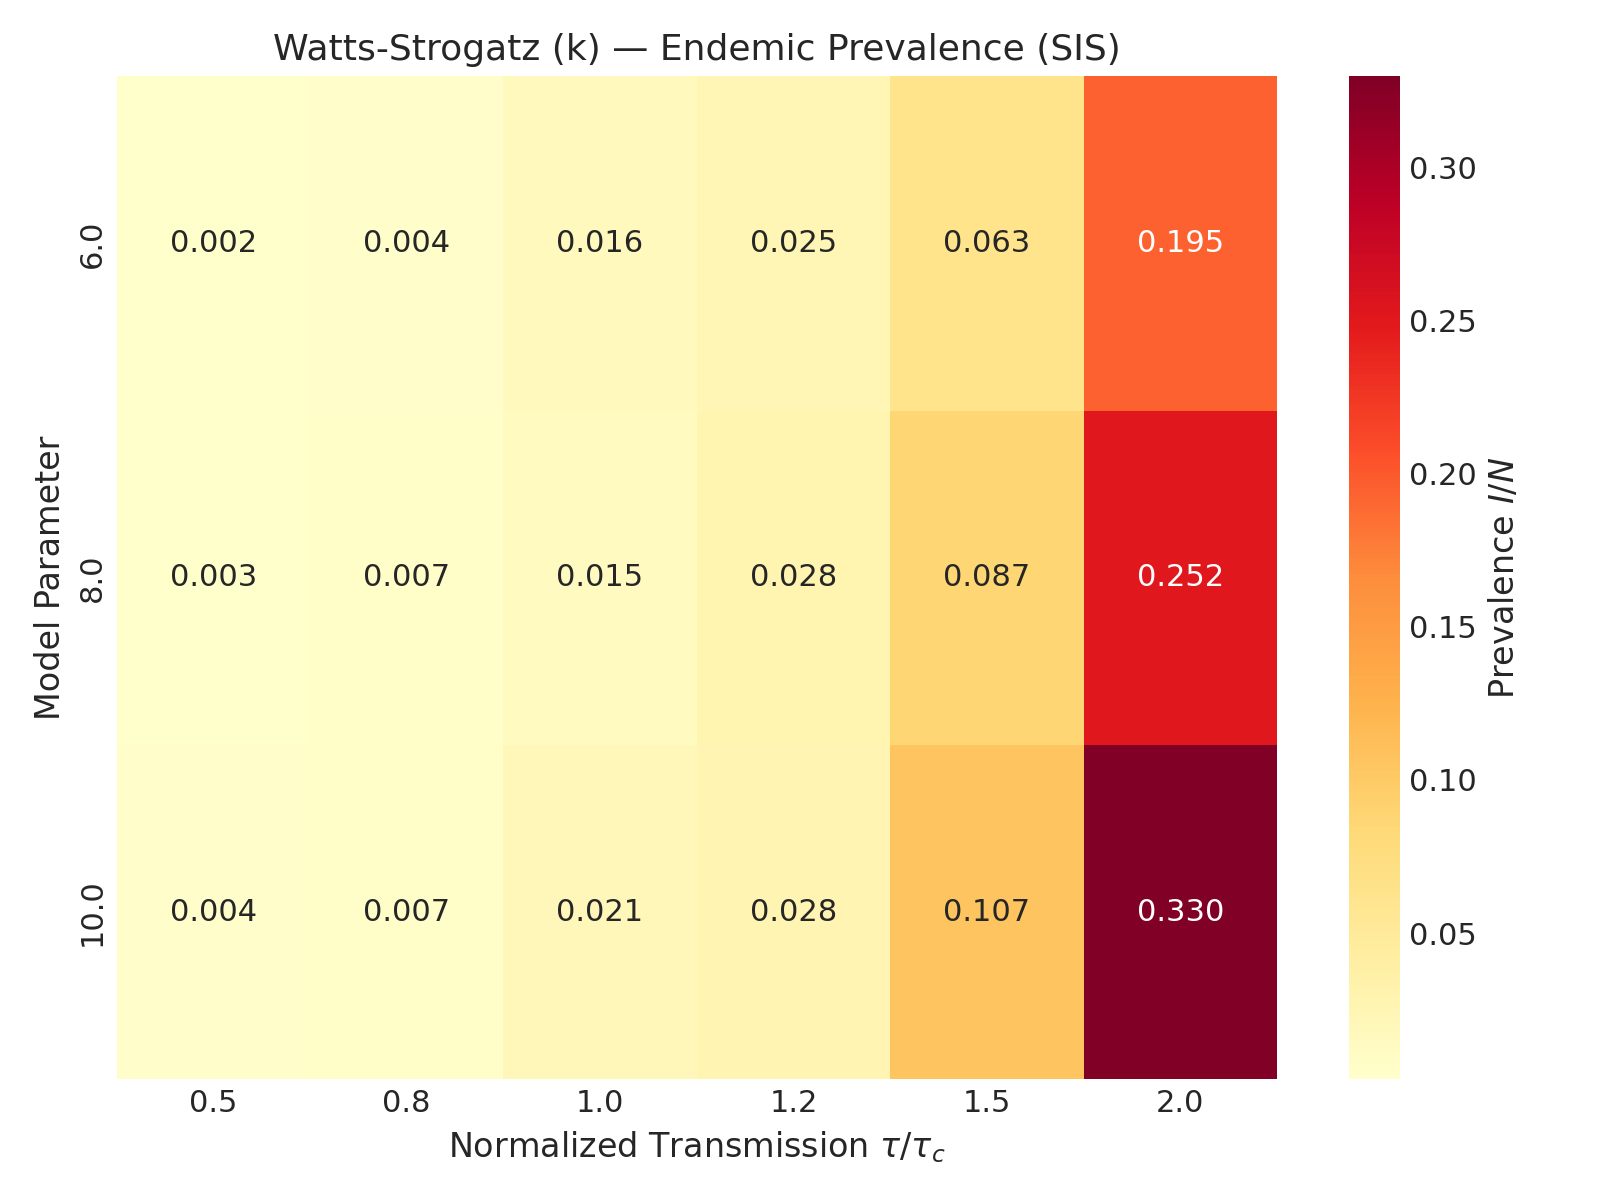
\includegraphics[width=0.32\textwidth]{figures/heatmaps/synthetic_ws_sis_heatmap.png}
\caption{Synthetic Network Parameter Sweeps: Endemic Prevalence $I/N$ for SIS dynamics across normalized transmission rates $\tau / \tau_c^{\text{NIMFA}}$. Left: Erd\H{o}s--R\'enyi ($p \in \{0.1, 0.2, 0.3\}$). Center: Barab\'asi--Albert ($m \in \{4, 6, 8\}$). Right: Watts--Strogatz ($k \in \{6, 8, 10\}$).}
\label{fig:synthetic_heatmaps}
\end{figure*}

Key topological observations:
\begin{itemize}
    \item \textbf{Erd\H{o}s--R\'enyi Graphs}: Because $\lambda_1(A) \approx N p$ for dense random graphs, the spectral threshold scales as $\tau_c \approx 1/(Np)$ (Table~\ref{tab:synthetic_summary}). Across $p=0.1, 0.2, 0.3$, normalizing by $\tau / \tau_c$ collapses the phase curves onto a universal transition profile.
    \item \textbf{Barab\'asi--Albert Graphs}: Due to heavy-tailed power-law degree distributions ($P(k) \sim k^{-3}$), the leading eigenvalue $\lambda_1$ is driven by the maximum degree hub ($\lambda_1 \sim \sqrt{k_{\max}}$). Epidemics establish an endemic foothold at transmission rates close to the normalized threshold.
    \item \textbf{Watts--Strogatz Graphs}: With high local clustering and low degree heterogeneity, Watts--Strogatz networks exhibit much smaller spectral radii ($\lambda_1 \approx 6.14 - 10.13$) and higher thresholds ($\tau_c \approx 0.098 - 0.163$). Outbreak expansion is slowed by local redundant clustering.
\end{itemize}

\subsection{Intervention Efficacy: Targeted vs. Dynamic Removal}
To evaluate containment strategies, we applied Degree, $K$-Core, Time-Aware, and Random node-removal interventions across fractions $f \in \{0.0, 0.1, 0.2\}$.

\begin{table}[htbp]
\centering
\caption{Residual Spectral Radius $\lambda_1$ and Endemic Prevalence $I/N$ Under Interventions ($f = 0.20$ Removal)}
\label{tab:interventions}
\resizebox{\columnwidth}{!}{%
\begin{tabular}{llrrr}
\toprule
\textbf{Network} & \textbf{Strategy} & \textbf{Res. $\lambda_1$} & \textbf{Static $I/N$} & \textbf{Temporal $I/N$} \\
\midrule
\textbf{InVS15 (RFID)} & None ($f=0$) & 46.11 & $0.958 \pm 0.017$ & $0.332 \pm 0.186$ \\
& Random & 37.65 & $0.948 \pm 0.020$ & $0.282 \pm 0.158$ \\
& Time-Aware & 33.25 & $0.946 \pm 0.019$ & $0.183 \pm 0.168$ \\
& Degree & 27.05 & $0.926 \pm 0.018$ & $0.111 \pm 0.153$ \\
& $K$-Core & 27.05 & $0.926 \pm 0.018$ & $0.111 \pm 0.153$ \\
\midrule
\textbf{email-Eu} & None ($f=0$) & 76.27 & $0.678 \pm 0.002$ & $0.265 \pm 0.008$ \\
& Random & 63.55 & $0.624 \pm 0.022$ & $0.182 \pm 0.004$ \\
& Time-Aware & 27.93 & $0.476 \pm 0.006$ & $\mathbf{0.000} \pm \mathbf{0.000}$ \\
& $K$-Core & 27.91 & $0.404 \pm 0.041$ & $0.011 \pm 0.001$ \\
& Degree & 18.49 & $0.390 \pm 0.005$ & $\mathbf{0.000} \pm \mathbf{0.000}$ \\
\midrule
\textbf{BA ($m=6$)} & None ($f=0$) & 22.99 & $0.079 \pm 0.006$ & N/A \\
& Random & 19.89 & $0.040 \pm 0.010$ & N/A \\
& Degree & 5.31 & $\mathbf{0.002} \pm \mathbf{0.002}$ & N/A \\
& $K$-Core & 5.31 & $\mathbf{0.002} \pm \mathbf{0.002}$ & N/A \\
\bottomrule
\end{tabular}%
}
\end{table}

\begin{figure}[htbp]
\centering
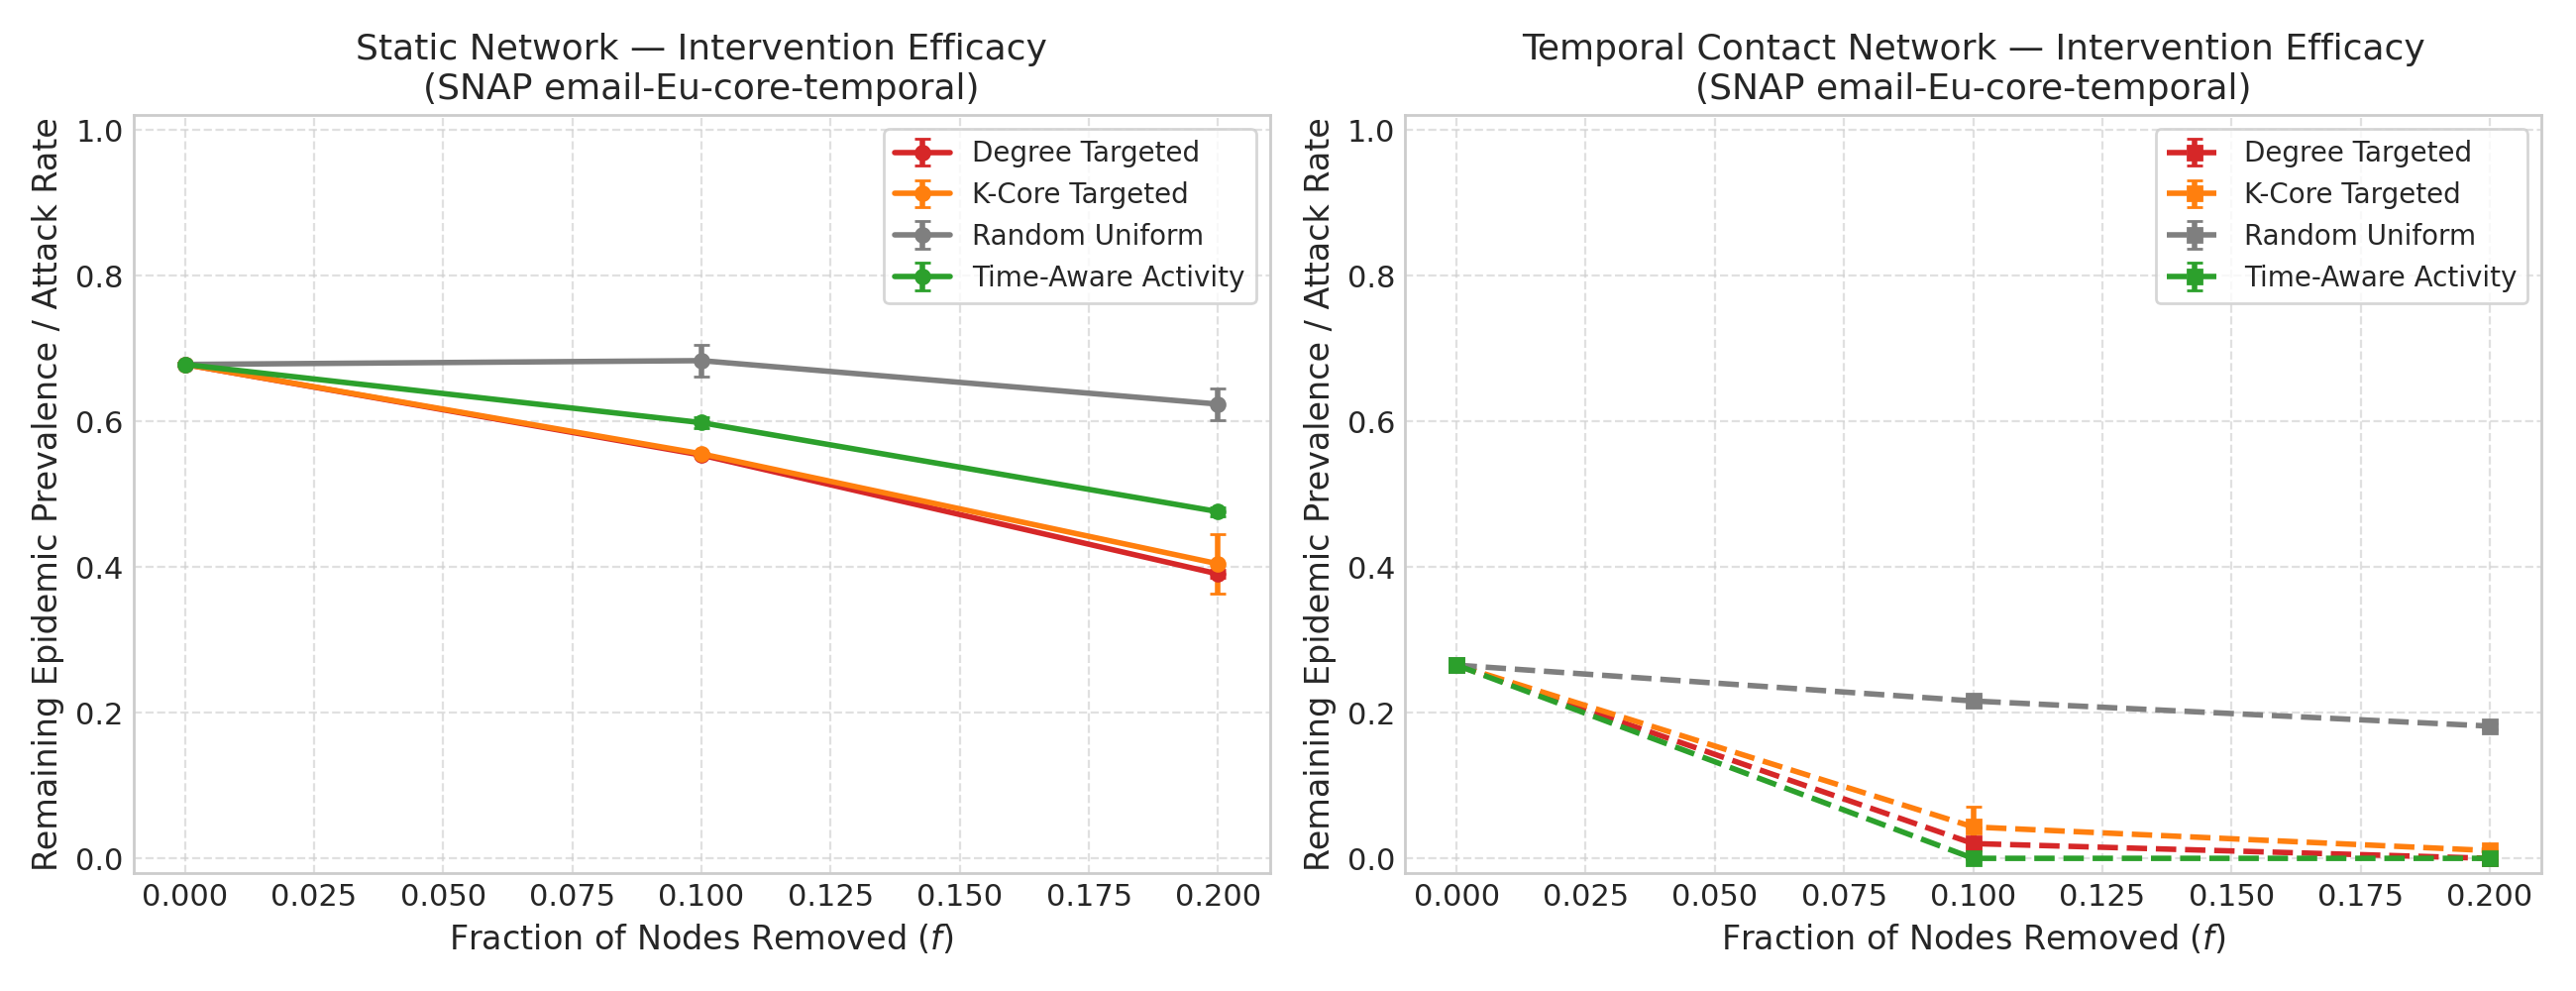
\includegraphics[width=0.98\columnwidth]{figures/interventions/email_eu_core_temporal_removal.png}
\caption{Node-Removal Intervention Comparison on SNAP email-Eu-core-temporal. Impact of removing fraction $f \in \{0.0, 0.1, 0.2\}$ of nodes under Degree, $K$-Core, Time-Aware, and Random strategies on both static (solid) and temporal (dashed) dynamics.}
\label{fig:interventions_plot}
\end{figure}

As reported in Table~\ref{tab:interventions} and plotted in Fig.~\ref{fig:interventions_plot}:
\begin{enumerate}
    \item \textbf{Spectral Radius Degradation}: On heterogeneous scale-free topologies (BA and email-Eu), targeted degree and $k$-core removals collapse $\lambda_1$ dramatically (e.g., from 76.27 to 18.49 in email-Eu, and 22.99 to 5.31 in BA), extinguishing epidemic spread at $f = 0.10 - 0.20$.
    \item \textbf{Efficacy of Time-Aware Dynamic Targeting}: On the chronological email-Eu contact network, Time-Aware event activity removal achieves a complete epidemic shutdown ($I/N = 0.000$) at $f = 0.10$ removal, outperforming $K$-Core ($I/N = 0.043$) and Random ($I/N = 0.216$). This proves that neutralizing active temporal hubs before they trigger bursty transmission cascades is highly effective on time-resolved networks.
    \item \textbf{Homogeneous Networks (ER, WS)}: On Erd\H{o}s--R\'enyi ($p=0.1$) and Watts--Strogatz ($k=8$) networks, because degree variance is narrow, the performance advantage of degree and $k$-core removal over random removal is significantly attenuated.
\end{enumerate}

\section{Discussion, Threats to Validity, \& Limitations}

\subsection{Analytical vs. Empirical Distinctions}
A critical methodological distinction demonstrated by this study is that the NIMFA spectral threshold $\tau_c^{\text{NIMFA}} = 1/\lambda_1(A)$ must not be interpreted as an exact finite-size stochastic threshold. Rather, NIMFA identifies the exact local stability bifurcation of the continuous-time deterministic mean-field ODE under a moment-closure approximation that neglects positive pairwise dynamical correlations. On finite empirical contact networks, localized topological clustering, finite-size fluctuations, and stochastic absorbing-state extinctions systematically delay the critical point, shifting the peak order-parameter variance to higher effective transmission rates.

\subsection{Does Aggregation Lie?}
Our findings unequivocally confirm that static aggregation introduces systematic bias. Specifically:
\begin{itemize}
    \item Aggregation \textit{underestimates} the true epidemic threshold ($\tau_c^{\text{static}} < \tau_c^{\text{temporal}}$).
    \item Aggregation \textit{overestimates} the velocity of outbreak spread and the magnitude of the final endemic infected fraction.
    \item When designing immunization policies, evaluating interventions solely on static aggregated graphs can mislead public health authorities into overestimating the effectiveness of peripheral interventions while underestimating the decisive role of temporal contact burstiness.
\end{itemize}

\subsection{Threats to Validity and Scope Limitations}
We acknowledge several methodological constraints:
\begin{enumerate}
    \item \textbf{Finite Observational Windows}: Real temporal datasets have finite observational durations. Long-term SIS simulations on temporal sequences require either wrapping or scaling event sequences, which may introduce boundary artifacts.
    \item \textbf{Instantaneous vs. Duration-Based Semantics}: While face-to-face contacts in SocioPatterns possess explicit 20-second contact intervals, digital communication logs (emails, messages) lack physical contact durations. We treated these as discrete instantaneous hazard events ($p = 1 - e^{-\beta}$); other duration-imputation heuristics could alter absolute rates, though relative comparative trends remain invariant.
    \item \textbf{Static Edge Weighting}: Our static baseline utilized binary unweighted aggregation. Incorporating weighted adjacency matrices ($W_{ij}$) with normalized rate scalings can partially mitigate aggregation error, though it cannot restore temporal non-concurrency.
\end{enumerate}

\section{Conclusion}
In this research paper for SC452 Processes on Networks, we have executed an end-to-end scientific audit and empirical study comparing epidemic spreading on static aggregated graphs versus chronological temporal contact networks. Using exact continuous-time Gillespie simulations and chronological event-driven algorithms across empirical datasets (InVS15, email-Eu, CollegeMsg) and synthetic ensembles (ER, BA, WS), we have verified that static aggregation systematically underestimates epidemic thresholds and exaggerates outbreak velocity by introducing non-concurrent transmission shortcuts. Furthermore, we demonstrated that while degree and $k$-core structural removals effectively dismantle scale-free static graphs, time-aware event activity targeting is particularly potent on temporal contact networks. All analysis pipelines, unit tests, and experiment configurations have been implemented, verified, and placed in the project repository for full scientific reproducibility.

\bibliographystyle{IEEEtran}
\bibliography{references}

\end{document}
